
\def\layersep{2.5cm}

\begin{figure}[!htb]
\centering	

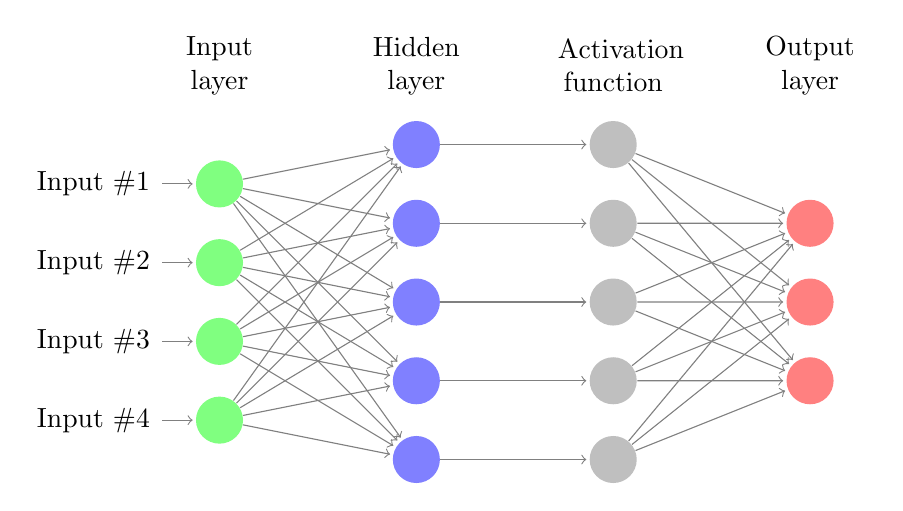
\begin{tikzpicture}[shorten >=1pt,->,draw=black!50, node distance=\layersep]
    \tikzstyle{every pin edge}=[<-,shorten <=1pt]
    \tikzstyle{neuron}=[circle,fill=black!25,minimum size=17pt,inner sep=0pt]
    \tikzstyle{input neuron}=[neuron, fill=green!50];
    \tikzstyle{output neuron}=[neuron, fill=red!50];
    \tikzstyle{hidden neuron}=[neuron, fill=blue!50];
    \tikzstyle{activation neuron}=[neuron, fill=gray!50];
    \tikzstyle{annot} = [text width=4em, text centered]

    % Draw the input layer nodes
    \foreach \name / \y in {1,...,4}
    % This is the same as writing \foreach \name / \y in {1/1,2/2,3/3,4/4}
        \node[input neuron, pin=left:Input \#\y] (I-\name) at (0,-\y) {};

    % Draw the hidden layer nodes
    \foreach \name / \y in {1,...,5}
        \path[yshift=0.5cm]
            node[hidden neuron] (H-\name) at (\layersep,-\y cm) {};
            
     % Draw the Activation Function layer nodes
     \foreach \name / \y in {1,...,5}
	     \path[yshift=0.5cm]
		     node[activation neuron] (A-\name) at (2*\layersep,-\y cm) {};

     % Draw the Activation Function layer nodes
     \foreach \name / \y in {1,...,3}
        \path[yshift=-0.5cm]
	     node[output neuron] (O-\name) at (3*\layersep,-\y cm) {};

    % Connect every node in the input layer with every node in the
    % hidden layer.
    \foreach \source in {1,...,4}
        \foreach \dest in {1,...,5}
            \path (I-\source) edge (H-\dest);

	\foreach \source in {1,...,5}
		\foreach \dest in {\source}
			\path (H-\source) edge (A-\dest);
			
    % Connect every node in the hidden layer with the output layer
    \foreach \source in {1,...,5}
	    \foreach \dest in {1,...,3}
	        \path (A-\source) edge (O-\dest);

    % Annotate the layers
    \node[annot,above of=H-1, node distance=1cm] (hl) {Hidden layer};
    \node[annot,right of=hl] (af) {Activation function};
    \node[annot,left of=hl] {Input layer};
    \node[annot,right of=af] {Output layer};
\end{tikzpicture}
\caption{Multi-Layer Perceptron}
\label{fig:multilayerPerceptron}
\end{figure}
